\subsubsection{Изолирование памяти}
\begin{frame}{\insertsubsubsection}

  \begin{figure}[h]
    \begin{tikzpicture}[
      align = center,
      ->,
      > = Stealth,
      thick,
      block/.style = {
        rectangle,
        draw,
        text = White,
        minimum width = 14cm,
        text width = 14cm,
        minimum height = 1.5cm,
        text centered,
      },
      ]

      \node[block, fill = ForestGreen] (user) {
        Пользовательское пространство
      };

      \node[block, below = 2 of user, fill = Maroon] (kernel) {
        Пространство операционной системы (ядра ОС)
      };

      \draw[double, <->] (user) -- node[right] {Интерфейс системных вызовов} (kernel);

    \end{tikzpicture}
    \caption{Система изолирования памяти}\label{fig:userspace_kernel_space}
  \end{figure}

  \note{

    Так как мультипроцессорная обработка данных становится всё популярнее, то и
    \textbf{задача изолирования памяти различных процессов} также становится
    актуальнее.

    Существует программная изоляция в виде разделения на
    \textbf{пользовательское пространство} и \textbf{пространство} операционной
    системы (\textbf{ядра ОС}).

  }
\end{frame}

\begin{frame}{\insertsubsubsection}

  \begin{figure}[h]
    \begin{tikzpicture}[
      align = center,
      ->,
      > = Stealth,
      thick,
      block/.style = {
        rectangle,
        draw,
        text = White,
        text centered,
      },
      ]

      \node (cat) {
        \texttt{\$ cat /proc/self/maps}
      };

      \node[block,
      font = \ttfamily,
      rectangle split,
      rectangle split parts = 9,
      rectangle split part fill = {
        Maroon, Maroon, Maroon,
        ForestGreen, ForestGreen, ForestGreen,
        PineGreen, ForestGreen, ForestGreen},
      below = of cat,
      ] (virt) {
        0xffff\_ffff\_1234\_0000
        \nodepart{two}
        $\cdots$
        \nodepart{three}
        0xffff\_ffff\_1200\_00c0
        \nodepart{four}
        $\cdots$
        \nodepart{five}
        0x7f90\_00c9\_8000
        \nodepart{six}
        $\cdots$
        \nodepart{seven}
        0x7ffc\_8f5b\_8000
        \nodepart{eight}
        $\cdots$
        \nodepart{nine}
        0x5637\_6a5f\_3000
      };

      \node[right = of virt.seven east] (vdso) {
        VDSO \\
        (Virtual Dynamic Shared Object)
      };

      \draw[->] (vdso) -- (virt.seven east);

    \end{tikzpicture}
    \caption{Пример карты памяти для процесса
      \texttt{cat}}\label{fig:cat_memory_map}
  \end{figure}

  \note{

    Также на первых порах была введена такая технология, как \textbf{виртуальная
      память}, которая представляла из себя \textbf{изолированные сегменты,
      ссылающиеся на физическую память}. На уровне виртуальной памяти
    операционная система могла иметь определённые права доступа к конкретному
    сегменту по конкретному смещению. Соответственно, \textbf{различные
      процессы} использовали \textbf{различные сегменты виртуальной памяти}.

  }
\end{frame}

\againframe<4>{core_elements}

\subsubsection{Трансляция адресов}
\begin{frame}{\insertsubsubsection}

  \begin{figure}[h]
    \begin{tikzpicture}[
      align = center,
      ->,
      > = Stealth,
      thick,
      block/.style = {
        rectangle,
        draw,
        fill = ForestGreen,
        text = White,
        text centered,
      },
      ]

      \node[block] (proc_a) {
        Процесс \\
        A
      };

      \node[
      block,
      below = 2.5cm of proc_a,
      ] (proc_b) {
        Процесс \\
        B
      };

      \node[rectangle,
      draw,
      text = White,
      rectangle split,
      rectangle split parts = 4,
      fill = ForestGreen,
      right = 2cm of proc_a,
      label = above:Виртуальные адреса A,
      ] (virt_a) {
        0x2134\_0000
        \nodepart{two}
        0x2134\_1000
        \nodepart{three}
        0x2134\_2000
        \nodepart{four}
        0x2134\_3000
        \nodepart{five}
      };

      \node[rectangle,
      draw,
      text = White,
      rectangle split,
      rectangle split parts = 4,
      fill = ForestGreen,
      right = 2cm of proc_b,
      label = above:Виртуальные адреса B,
      ] (virt_b) {
        0x4114\_0000
        \nodepart{two}
        0x4114\_1000
        \nodepart{three}
        0x4114\_2000
        \nodepart{four}
        0x4114\_3000
        \nodepart{five}
      };

      \node[
      right = 2.5cm of $(virt_a)!0.5!(virt_b)$,
      draw,
      fill = ForestGreen!60,
      minimum width = 1cm,
      minimum height = 6cm,
      label = above:TLB,
      ] (tlb) {};

      \node[rectangle,
      draw,
      text = White,
      rectangle split,
      rectangle split parts = 8,
      rectangle split part fill = {
        ForestGreen, ForestGreen, ForestGreen, PineGreen,
        ForestGreen, ForestGreen, ForestGreen, ForestGreen
      },
      right = 5cm of $(virt_a)!0.5!(virt_b)$,
      label = above: Физические адреса,
      ] (phys) {
        0x7000
        \nodepart{two}
        0x6000
        \nodepart{three}
        0x5000
        \nodepart{four}
        0x4000
        \nodepart{five}
        0x3000
        \nodepart{six}
        0x2000
        \nodepart{seven}
        0x1000
        \nodepart{eight}
        0x0000
        \nodepart{nine}
      };

      \path (proc_a)          edge (virt_a.one)
            (proc_a)          edge (virt_a.two)
            (proc_a)          edge (virt_a.three)
            (proc_a)          edge (virt_a.four)
            (proc_b)          edge (virt_b.one)
            (proc_b)          edge (virt_b.two)
            (proc_b)          edge (virt_b.three)
            (proc_b)          edge (virt_b.four)

            (virt_a.one east)   edge (phys.two)
            (virt_a.two east)   edge (phys.eight)
            (virt_a.three east) edge (phys.six)
            (virt_a.four east)  edge (phys.one)
            (virt_b.one east)   edge (phys.three)
            (virt_b.two east)   edge (phys.seven)
            (virt_b.three east) edge (phys.four)
            (virt_b.four east)  edge (phys.four);

    \end{tikzpicture}
    \caption{Пример трансляции адресов (0x4000 --- разделяемая страница
      памяти)}\label{fig:address_translation}
  \end{figure}

  \note{

    В итоге существует \textbf{два понятия}: \textbf{виртуальный адрес} памяти,
    который доступен процессу и \textbf{физический адрес} памяти, по которому
    процесс напрямую обращаться не может.

    Вместо сегментов памяти, современные процессоры используют так называемые
    \textbf{страницы памяти}, которые представляют из себя \textbf{участки
      памяти фиксированного размера}. И виртуальная, и физическая память
    разбивается на подобные страницы, при этом страницы виртуальной памяти
    ссылаются на страницы физической с помощью указания номеров требуемых
    страниц. Размеры страниц памяти в современных процессорах варьируются, но
    самыми маленькими обычно являются страницы \textbf{размером 4KB или 1KB}.
    Страницы физической и виртуальной памяти выровнены \textbf{в соответствии с
      их размером}, т. е. страница физической памяти размером в 4KB выровнена со
    страницей виртуальной памяти такого же размера.

  }
\end{frame}

% \begin{frame}{\insertsubsubsection. x86-64}

%   \begin{figure}[h]
%     \begin{tikzpicture}[
%       align = center,
%       ->,
%       > = Stealth,
%       thick,
%       double = ForestGreen,
%       block_split/.style = {
%         rectangle,
%         rectangle split,
%         rectangle split parts = 6,
%         draw,
%         % fill = ForestGreen,
%         text = White,
%         text centered,
%         font = \scriptsize,
%       },
%       block/.style = {
%         rectangle,
%         draw,
%         fill = ForestGreen,
%         text = White,
%         text centered,
%       },
%       ]

%       \node[block] (reg) {
%         CR3
%       };

%       \node[block_split, right = of reg, label = above:PML4,
%       rectangle split part fill = {
%         ForestGreen, ForestGreen, ForestGreen, Blue, ForestGreen, ForestGreen
%       },
%       ] (pml4) {
%         PML4E 0
%         \nodepart{two}
%         PML4E 1
%         \nodepart{three}
%         $\cdots$
%         \nodepart{four}
%         \#PML4EI
%         \nodepart{five}
%         $\cdots$
%         \nodepart{six}
%         PML4E 511
%       };

%       \node[block_split, right = of pml4, label = above:PDPT,
%       rectangle split part fill = {
%         ForestGreen, ForestGreen, ForestGreen, Mahogany, ForestGreen, ForestGreen
%       },
%       ] (pdpt) {
%         PDPTE 0
%         \nodepart{two}
%         PDPTE 1
%         \nodepart{three}
%         $\cdots$
%         \nodepart{four}
%         \#PDPTEI
%         \nodepart{five}
%         $\cdots$
%         \nodepart{six}
%         PDPTE 511
%       };

%       \node[block_split, right = of pdpt, label = above:Page Directory,
%       rectangle split part fill = {
%         ForestGreen, ForestGreen, ForestGreen, PineGreen, ForestGreen, ForestGreen
%       },
%       ] (pd) {
%         PDE 0
%         \nodepart{two}
%         PDE 1
%         \nodepart{three}
%         $\cdots$
%         \nodepart{four}
%         PDE \#PDI
%         \nodepart{five}
%         $\cdots$
%         \nodepart{six}
%         PDE 511
%       };

%       \node[block_split, right = of pd, label = above:Page Table,
%       rectangle split part fill = {
%         ForestGreen, ForestGreen, ForestGreen, RoyalBlue, ForestGreen, ForestGreen
%       },
%       ] (pt) {
%         PTE 0
%         \nodepart{two}
%         PTE 1
%         \nodepart{three}
%         $\cdots$
%         \nodepart{four}
%         PTE \#PTI
%         \nodepart{five}
%         $\cdots$
%         \nodepart{six}
%         PTE 511
%       };

%       \node[block_split, right = of pt, label = above:4 KiB Page,
%       rectangle split part fill = {
%         ForestGreen, ForestGreen, ForestGreen, brown, ForestGreen, ForestGreen
%       },
%       ] (page) {
%         Byte 0
%         \nodepart{two}
%         Byte 1
%         \nodepart{three}
%         $\cdots$
%         \nodepart{four}
%         Offset
%         \nodepart{five}
%         $\cdots$
%         \nodepart{six}
%         Byte 4095
%       };

%       \node[draw,
%       text = White,
%       text centered,
%       rectangle split,
%       rectangle split horizontal,
%       rectangle split parts = 5,
%       below = of pd,
%       rectangle split part fill = {
%         Blue, Mahogany, PineGreen, RoyalBlue, brown
%       },
%       label = below:48-битный виртуальный адрес,
%       ] (virt) {
%         PML4I (9B)
%         \nodepart{two}
%         PDPTI (9B)
%         \nodepart{three}
%         PDI (9B)
%         \nodepart{four}
%         PTI (9B)
%         \nodepart{five}
%         Offset (12B)
%       };


%       \path (reg) edge (pml4.north west)
%       (pml4.four east) edge (pdpt.north west)
%       (pdpt.four east) edge (pd.north west)
%       (pd.four east) edge (pt.north west)
%       (pt.four east) edge (page.north west);

%     \end{tikzpicture}
%     \caption{Трансляция адресного пространства для страниц в 4KB на x86-64
%       процессорах}\label{fig:address_translation_tables}
%   \end{figure}

%   \note{

%     Массив, который отображает 48-битное пространство --- занимает 512GB, что
%     \textbf{не рационально}. Используется \textbf{многоуровневая трансляция}.

%     \texttt{CR3} регистр изменяется в соответствии с \textbf{контекстом}
%     выполнения, что обеспечивает \textbf{изоляцию}.

%     Современные процессоры Intel имеют 4 уровня трансляции адресов (см.
%     рисунок \ref{fig:address_translation_tables}]).

%     \begin{enumerate}
%     \item PML4 (page map level) --- 48-битное виртуальное адресное пространство
%       на 512 регионов по 512GB.
%     \item Таблица указателей директории страниц PDPT (page directory pointer
%       tables) --- на 512 записей по 1GB виртуальной памяти. Эта 1GB виртуальная
%       страница может напрямую ссылаться на 1GB страницу или страницу директорий
%       PD (page directory).
%     \item PD --- 512 ячеек по 2MB.
%     \item PT (page table) --- 4KB.
%     \end{enumerate}

%   }

% \end{frame}

% \begin{frame}{Трансляция адресов. ARM}

%   \begin{figure}[h]
%     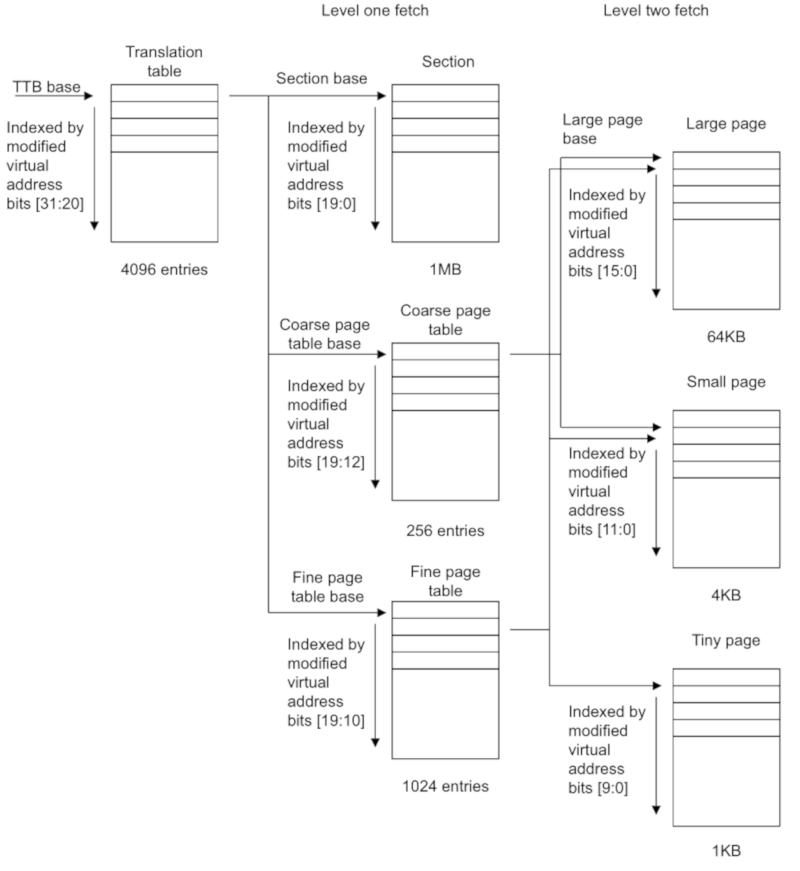
\includegraphics[height = 0.9\textheight]{arm_addr_transl}
%     \caption{Трансляция адресного пространства на ARMv5+
%       процессорах}\label{fig:armv5_addr_transl}
%   \end{figure}

%   \note{

%     Что касается ARM архитектуры, то там складывается похожая картина. Есть
%     несколько отличий: используются \textbf{отображения других размеров} (1MB
%     --- секции, 64KB --- большие страницы, 4KB --- маленькие страницы и 1KB ---
%     крошечные страницы, на поздних версиях большего размера); используется
%     регистр \texttt{c2} (часть \texttt{CP15} регистров) (\textbf{Translation
%       Table Base Register TTBR}) для получения указателя на таблицу в физическом
%     адресном пространстве, содержащую описания секции или страницы (или и того и
%     другого); в отличии от Intel используется \textbf{двухуровневая трансляция}
%     (см. рисунок \ref{fig:armv5_addr_transl}) и другие.

%     На современных ARM процессорах (Cortex-A) используется два регистра для
%     хранения физического адреса таблицы трансляции адресов (\texttt{TTBR0} и
%     \texttt{TTBR1}). Обычно один из них используется для
%     \textbf{пользовательского пространства}, а другой для \textbf{пространства
%       адресов ядра}. Это может служит причиной, почему некоторые атаки работают
%     на x86-64 процессорах, но \textbf{не работают на ARM}. При попытке доступа
%     из пользовательского контекста выполнения к регистру, который отвечает за
%     адресацию в ядерном пространстве, возникает исключение.

%   }

% \end{frame}
